\documentclass[tikz,border=10pt]{standalone}
\usepackage{tikz}
\usetikzlibrary{positioning, arrows.meta}

\begin{document}

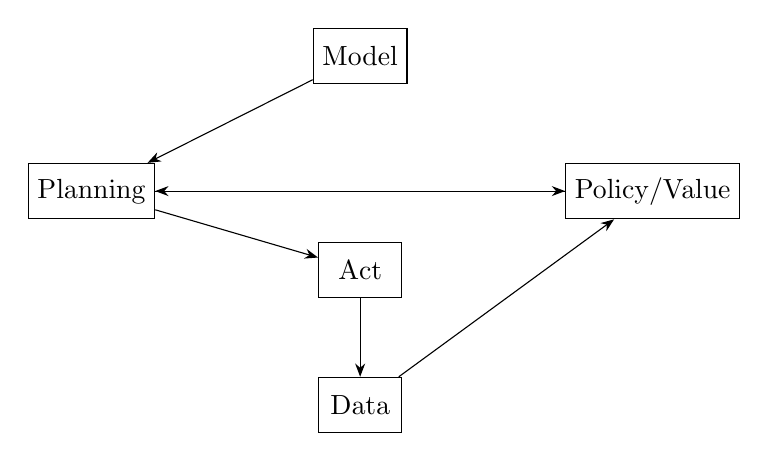
\begin{tikzpicture}[>=Stealth, node distance=1cm and 2cm, every node/.style={draw, rectangle, minimum height=2em, minimum width=3em, text centered}]
    % Nodes
    \node (model) {Model};
    \node (planning) [below left=of model] {Planning};
    \node (policy) [below right=of model] {Policy/Value};
    \node (act) [below=2cm of model] {Act};
    \node (data) [below=1cm of act] {Data};

    % Arrows
    \draw[->] (planning) -- (policy);
    \draw[->] (policy) -- (planning);
    \draw[->] (planning) -- (act);
    \draw[->] (data) -- (policy);
    \draw[->] (model) -- (planning);
    \draw[->] (act) -- (data);

\end{tikzpicture}

\end{document}
